% Proposed design: per-node metadata managers on BlueField-3 DPUs,
% node-local consistency, eventually consistent directory, lookups from the host scheduler,
% and recompute-while-loading (compute from the front, load from the back).
% Companion to request_path.tex (same styles and colours).
% Build: lualatex design_arch.tex   (system Helvetica via fontspec)
\documentclass{article}
\usepackage{fontspec}
\setsansfont{Helvetica}
\renewcommand{\familydefault}{\sfdefault}
\usepackage{tikz}
\usetikzlibrary{arrows.meta}
\pagestyle{empty}

\definecolor{rpc}{HTML}{B2182B}   % metadata messages
\definecolor{data}{HTML}{2166AC}  % KV data
\definecolor{compute}{gray}{0.30} % recomputation on the GPU
\definecolor{nodefill}{gray}{0.94}
\definecolor{subtext}{gray}{0.35}

\tikzset{
  nodebox/.style={draw=black, line width=0.6pt, rounded corners=2pt, fill=nodefill},
  dpubox/.style={draw=black, line width=0.6pt, rounded corners=1.5pt, fill=white},
  mgrbox/.style={draw=rpc!85!black, line width=0.8pt, rounded corners=1.5pt, fill=rpc!6},
  comp/.style={draw=black, line width=0.5pt, rounded corners=1.5pt, fill=white,
               align=center, inner sep=2pt},
  offpath/.style={comp, draw=black!40, text=black!55},
  ttl/.style={font=\footnotesize\bfseries},
  sub/.style={font=\scriptsize, text=subtext},
  step/.style={circle, fill=#1, text=white, font=\fontsize{6}{6}\selectfont\bfseries,
               inner sep=0pt, minimum size=9.5pt},
  metaline/.style={-{Stealth[length=4.5pt,width=3.8pt]}, line width=0.9pt, draw=rpc},
  dataline/.style={line width=1.6pt, draw=data},
  compline/.style={-{Stealth[length=6pt,width=5.5pt]}, line width=1.6pt, draw=compute},
  updline/.style={{Stealth[length=4pt,width=3.4pt]}-{Stealth[length=4pt,width=3.4pt]},
                  line width=0.6pt, draw=black!50, dash pattern=on 2.5pt off 1.5pt},
  blk/.style={draw=black!45, line width=0.4pt, fill=white, minimum size=0.26cm, inner sep=0pt},
  kvblk/.style={blk, fill=data, draw=data!70!black},
  cblk/.style={blk, fill=black!40, draw=black!65},
}

% #1 = x of the DPU centre, #2 = node letter
\newcommand{\dpu}[2]{%
  \draw[dpubox] (#1-2.0,0.3) rectangle (#1+2.0,5.85);
  \node[ttl] at (#1,5.6) {BlueField-3 DPU};
  \node[comp, fill=black!7, minimum width=3.7cm, minimum height=0.55cm] (nic#2) at (#1,4.85)
    {\footnotesize NIC};
  \draw[mgrbox] (#1-1.85,0.45) rectangle (#1+1.85,4.35);
  \node[anchor=north, align=center] at (#1,4.3)
    {\footnotesize\bfseries Metadata manager\\[-1pt]{\scriptsize\mdseries\color{subtext}Arm cores}};
  \node[comp, minimum width=3.4cm, minimum height=0.85cm] (idx#2) at (#1,2.95)
    {\footnotesize Local index + allocator\\[-1pt]{\scriptsize\color{subtext}authoritative for node #2}};
  \node[comp, minimum width=3.4cm, minimum height=0.85cm] (dir#2) at (#1,1.45)
    {\footnotesize Directory replica\\[-1pt]{\scriptsize\color{subtext}eventually consistent}};
}
% KV pool and host CPU: #1 = x of the column centre, #2 = node letter, #3 = host CPU role,
% #4 = host CPU box style
\newcommand{\hostcol}[4]{%
  \node[comp, minimum width=2.6cm, minimum height=1.35cm] (pool#2) at (#1,2.75) {};
  \node[anchor=north, align=center, inner sep=2.5pt] at (pool#2.north)
    {\footnotesize KV pool\\[-1pt]{\scriptsize\color{subtext}DRAM / SSD}};
  \foreach \c in {0,...,4} { \node[blk] (blk#2\c) at (#1-0.84+\c*0.42,2.375) {}; }
  \node[#4, minimum width=2.6cm, minimum height=1.0cm] (cpu#2) at (#1,0.85)
    {\footnotesize Host CPU\\[-1pt]{\scriptsize #3}};
}

\begin{document}
\setbox0=\hbox{%
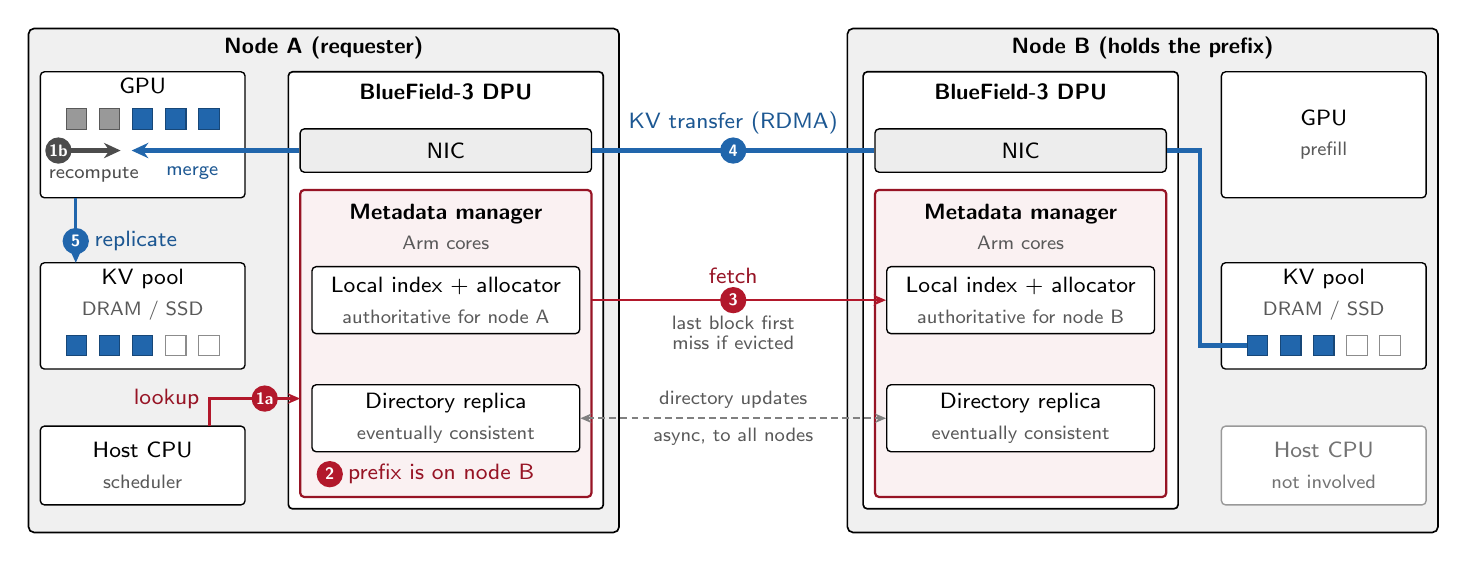
\begin{tikzpicture}[x=1cm,y=1cm]

  % --- Node A (requester) ------------------------------------------------------
  \draw[nodebox] (0,0) rectangle (7.5,6.4);
  \node[ttl] at (3.75,6.15) {Node A (requester)};
  \hostcol{1.45}{A}{\color{subtext}scheduler}{comp}
  \dpu{5.3}{A}
  % GPU: the prefix's KV is recomputed from the front and fetched from the back
  \node[comp, minimum width=2.6cm, minimum height=1.6cm] (gpuA) at (1.45,5.05) {};
  \node[font=\footnotesize, anchor=north, inner sep=2.5pt] at (gpuA.north) {GPU};
  \foreach \c in {0,1} { \node[cblk] at (0.61+\c*0.42,5.25) {}; }
  \foreach \c in {2,3,4} { \node[kvblk] at (0.61+\c*0.42,5.25) {}; }
  \node[font=\scriptsize, text=compute, anchor=north west, inner sep=1.5pt] at (0.2,4.7) {recompute};
  \node[font=\scriptsize, text=data!85!black, anchor=north, inner sep=1.5pt] at (2.08,4.7) {merge};

  % --- Node B (holds the prefix) -----------------------------------------------
  \draw[nodebox] (10.4,0) rectangle (17.9,6.4);
  \node[ttl] at (14.15,6.15) {Node B (holds the prefix)};
  \dpu{12.6}{B}
  \hostcol{16.45}{B}{not involved}{offpath}
  \node[comp, minimum width=2.6cm, minimum height=1.6cm] (gpuB) at (16.45,5.05)
    {\footnotesize GPU\\[-1pt]{\scriptsize\color{subtext}prefill}};
  \foreach \c in {0,1,2} { \node[kvblk] (kvB\c) at (blkB\c) {}; }

  % --- (1a) the scheduler sends the lookup to its own DPU -----------------------
  \draw[metaline] (2.3,1.35) -- (2.3,1.7) -- (3.45,1.7);
  \node[step=rpc] at (3.0,1.7) {1a};
  \node[font=\footnotesize, text=rpc!85!black, anchor=east, inner sep=1.5pt] at (2.23,1.7) {lookup};

  % --- (1b) at the same time, the GPU starts recomputing from the first block ---
  \draw[compline] (0.3,4.85) -- (1.17,4.85);
  \node[step=compute] at (0.38,4.85) {1b};

  % --- (2) the local directory replica names the holder -------------------------
  \node[font=\footnotesize, text=rpc!85!black, anchor=west, inner sep=1.5pt] (owner) at (4.0,0.74) {prefix is on node B};
  \node[step=rpc, anchor=east] at (owner.west) {2};

  % --- (3) one request to the holder's DPU --------------------------------------
  \draw[metaline] (7.15,2.95) -- (idxB.west);
  \node[step=rpc] at (8.95,2.95) {3};
  \node[font=\footnotesize, text=rpc!85!black, anchor=south, inner sep=2pt] at (8.95,3.08) {fetch};
  \node[sub, anchor=north, inner sep=2pt, align=center] at (8.95,2.82) {last block first\\[-1pt]miss if evicted};

  % --- (4) the holder's NIC writes the KV into the requester's GPU (RDMA) --------
  \draw[dataline] (kvB0.west) -| (14.88,4.85) -- (nicB.east);
  \draw[dataline] (nicB.west) -- (nicA.east);
  \draw[dataline, -{Stealth[length=6pt,width=5.5pt]}] (nicA.west) -- (1.31,4.85);
  \node[step=data] at (8.95,4.85) {4};
  \node[font=\footnotesize, text=data!85!black, anchor=south, inner sep=2pt] at (8.95,4.98) {KV transfer (RDMA)};

  % --- (5) the fetched blocks are replicated into the local pool (hot copy) ------
  \foreach \c in {0,1,2} { \node[kvblk] at (blkA\c) {}; }
  \draw[line width=1.1pt, draw=data, -{Stealth[length=4.5pt,width=4pt]}] (0.6,4.25) -- (0.6,3.425);
  \node[step=data] at (0.6,3.7) {5};
  \node[font=\footnotesize, text=data!85!black, anchor=west, inner sep=1.5pt] at (0.78,3.7) {replicate};

  % --- Directory updates between DPUs, off the critical path ---------------------
  \draw[updline] (dirA.east) -- (dirB.west);
  \node[sub, anchor=south, inner sep=2pt] at (8.95,1.5) {directory updates};
  \node[sub, anchor=north, inner sep=2pt] at (8.95,1.4) {async, to all nodes};

\end{tikzpicture}}%
\pdfvariable horigin=0pt
\pdfvariable vorigin=0pt
\pagewidth=\dimexpr\wd0+8pt\relax
\pageheight=\dimexpr\ht0+\dp0+8pt\relax
\shipout\vbox{\kern4pt\hbox{\kern4pt\box0\kern4pt}\kern4pt}
\end{document}
